\kafkasection{Program \texttt{Percolation} generates percolation configurations on the square lattice. The program computes $P_\infty(p)$, the fraction of states in the spanning cluster; $S(p)$, the mean number of sites in the finite clusters; $P_{span}(p)$, the probability of a spanning cluster; and $n_s$, the number of clusters with $s$ sites for various values of $p$. The clusters are shown at the default value $p=0.5927$, and the largest cluster is shown in red.}
\kafkasubsection{Run the program and look at the configurations. A spanning cluster is defined as one that
connects the top and bottom of the lattice and the left and right boundaries. How would you
describe the structure of the spanning clusters at $p = 0.8$? Are the clusters compact with few
holes or ramified and stringy?}
The clusters definitely align with the compact description as we see little holes and structure spanning the whole field.

\kafkasubsection{Visually inspect the configurations at $p = p_c \approx 0.5927$. How would you describe the spanning clusters at the percolation threshold? Increase the size of the lattice. Do the spanning clusters become less dense? Note that there are clusters of all sizes at $p = pc$.}
We see smaller structures with branching behavior and defined borders. "ramified and stringy" if you will. When we increase the size of the lattice, we see less dense structures as the holes within them become larger, scaling with the size of the system.
\kafkasubsection{Run the program for at least 100 trials and look at the log-log plot of the cluster size distribution $n_s$ versus $s$ at $p=p_c$. Do you see linear behavior for some range of values of $s$? What functional form does this linear dependence suggest? Choose \texttt{Data Table} under the \texttt{Views} menu and fit your data to the form $n_s$ = $As^{-\tau}$, Where $A$ and $\tau$ are fitting parameters. The exact result for $\tau$ in $d=2$ is given in Table 9.2 How does your estimate for $\tau$ compare?}
Yes, we see linear behavior. Because this is a log-log plot, a linear behavior indicates some power law with a given exponent. I used scipy's \texttt{curve\_fit} function which returned a fit of $\tau = 2.03$. This is close to the literature value of $\tau = 187/91 \approx 2.05$.
\kafkasubsection{Choose $p=0.4$ and 0.8 and look at the log-log plots of the cluster size distribution $n_s$ versus $s$. Is the qualitative behavior of $n_s$ for large $s$ the same as it is at $p=p_c$?}
At the lower value of $p=0.4$, we see a deviation from linear behavior at higher $s$. The curve slightly dips down with accelerating slope. For the higher $p=0.8$ value, the cluster size distribution drops quickly as well.
\kafkasubsection{Choose $L=128$ and do atleast 100 trials (1000 is better) at various values of $p$ near $p_c$. Copy the data for $S(p)$ and $P_\infty(p)$ and make a log-log plot of $S(p)$ and $P_\infty(p)$ versus $p-p_c$. There should be a region of your plot that is linear, indicating a possible power law. We will estimate the critical exponents $\beta$ and $\gamma$ in the next problem.}
\begin{figure}[H]
    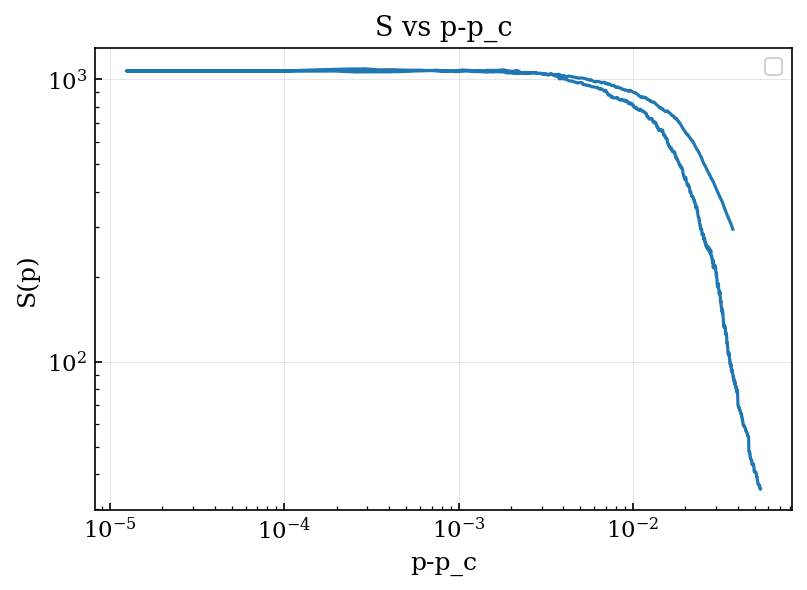
\includegraphics[width= 0.5\linewidth]{S1e.png}
    \centering
\end{figure}
\begin{figure}[H]
    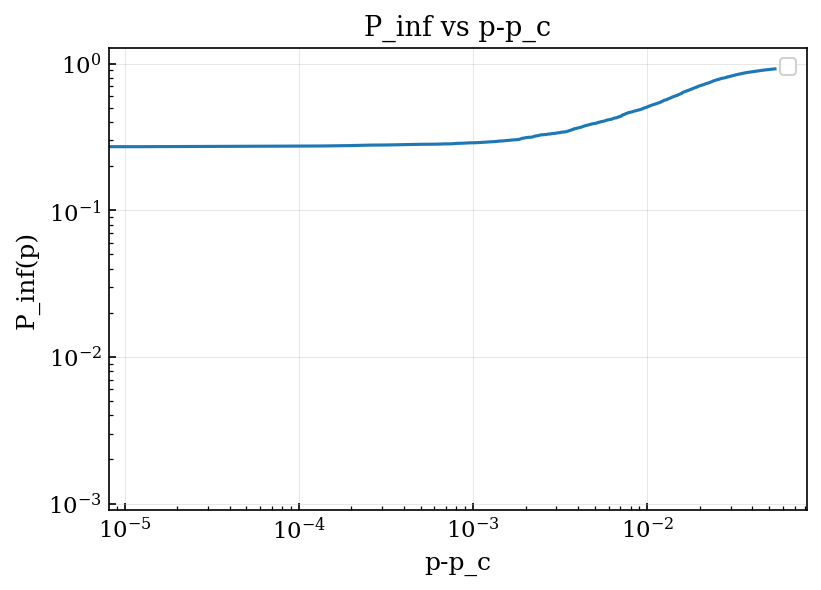
\includegraphics[width= 0.5\linewidth]{pinf1e.png}
    \centering
\end{figure}
We see linear behavior for the values close to $p_c$.